% Please use the skeleton file you have received in the
% invitation-to-submit email, where your data are already
% filled in. Otherwise please make sure you insert your
% data according to the instructions in PoSauthmanual.pdf
\documentclass{PoS}
\usepackage[utf8x]{inputenc}
\usepackage{wrapfig}\usepackage{wrapfig} % Allows wrapping text around tables and figures
\usepackage{graphicx}
\usepackage{subcaption}
\usepackage{float}
\newcommand{\bbbar}{$b\bar{b}$}
\newcommand{\afb}{$A_{FB}^b$}
\newcommand{\sm}{Standard Model}
\newcommand{\bsm}{Beyond Standard Model}
\newcommand{\mF}{\mathcal{F}^I} % Allows wrapping text around tables and figures

%\usepackage{wrapfig}

\usepackage{lineno}
\usepackage{array}
\usepackage{lscape}
\usepackage{graphicx}
\usepackage{subcaption}
\usepackage{float}
\usepackage{multicol} % This is so we can have multiple columns of text side-by-side
\usepackage{amsmath}
\columnsep=100pt % This is the amount of white space between the columns in the poster
\columnseprule=3pt % This is the thickness of the black line between the columns in the poster

\usepackage[svgnames]{xcolor} % Specify colors by their 'svgnames', for a full list of all colors available see here: http://www.latextemplates.com/svgnames-colors

\usepackage{times} % Use the times font
%\usepackage{palatino} % Uncomment to use the Palatino font

\usepackage{graphicx} % Required for including images
\graphicspath{{figures/}} % Location of the graphics files
\usepackage{booktabs} % Top and bottom rules for table
\usepackage[font=small,labelfont=bf]{caption} % Required for specifying captions to tables and figures
\usepackage{amsfonts, amsmath, amsthm, amssymb} % For math fonts, symbols and environments
\usepackage{wrapfig} % Allows wrapping text around tables and figures

\newcommand{\bbbar}{$b\bar{b}$}
\newcommand{\afb}{$A_{FB}^b$}
\newcommand{\sm}{Standard Model}
\newcommand{\bsm}{Beyond Standard Model}
\newcommand{\mF}{\mathcal{F}^I}

\title{Studies of $ e^+e^-\to b\bar{b}$ channel at the International Linear Collider}

\ShortTitle{Studies of $ e^+e^-\to b\bar{b}$ channel at the International Linear Collider}

\author{\speaker{Sviatoslav BILOKIN}\\%thanks{A footnote may follow.}\\
        Laboratoire de l'Acceler\'ateur Lin\'eare\\
        E-mail: \email{bilokin@lal.in2p3.fr}}

\author{Roman P\"OSCHL\\
        Laboratoire de l'Acceler\'ateur Lin\'eare\\
        E-mail: \email{poeschl@lal.in2p3.fr}}

\author{Fran\c cois RICHARD\\
	Laboratoire de l'Acceler\'ateur Lin\'eare\\
	E-mail: \email{richard@lal.in2p3.fr}}

\abstract{
	The heavy quark doublet plays a central role in the quest for new physics. The complementarity between studies of electroweak top quark production and bottom quark production is therefore intuitively clear and pointed out in the literature.
	The tension between the LEP measurement and the Standard Model prediction of the forward-backward asymmetry \afb\ is still one of the unsolved questions in the field and may be interpreted as a first manifestation of New Physics in the heavy quark sector. The process $e^+e^-\to b\bar{b}$ at the ILC offers a unique opportunity for a final word on the tension. Polarised beams allow for a large disentangling of the coupling constants or form factors that govern the $Z^0/\gamma b \bar{b}$ vertex.
	
	%These studies are based on a detailed simulation study of the process $e^+e^-\to b\bar{b}$ at 250\,GeV with the ILD Detector. Besides the phenomenological implications, the studies demonstrate that with a careful analysis of the final state the charge of the b-quarks can be determined on an event-by-event basis with the ILD Detector. Such a capability is unprecedented by past and present particle physics experiments.
	}

\FullConference{EPS-HEP 2017, European Physical Society conference on High Energy Physics\\
		5-12 July 2017\\
		Venice, Italy}

\begin{document}

\section{Introduction}
So far, LEP~I has determined the b-quark couplings to the $Z^0$ boson by measuring the b partial width and the forward-backward asymmetry called \afb. These quantities provide the most precise value of $\sin^2\theta_W$ at LEP~I. It turns out that this value is at about three standard deviation away from the very precise value from SLD using beam polarization~\cite{bib:AfbSMFit}. Redoing precisely this measurement is therefore a priority for future $e^+e^-$ colliders. 

In this study, we intend to prove that the International Linear Collider~\cite{bib:ILC}, with {polarized beams and high luminosity}, offers a unique opportunity for precise measurements well above the resonance, where both $Z^0$ and photon exchanges are present. 
This additional complexity may turn up to be of a great advantage since it allows, through $\gamma - Z^0$ interference, to be sensitive to the sign of $Z^0$ couplings and fully solve the LEP~I puzzle in an unambiguous way. 
Recall that the LEP~I anomaly can be interpreted up to a sign ambiguity for what concerns the right-handed coupling $Z^0 b\bar{b}$, referred hereafter as $g_R^Z$, which shows the largest deviation~\cite{bib:RSTOP}.

%\begin{figure}[h]
%	{\centering
%		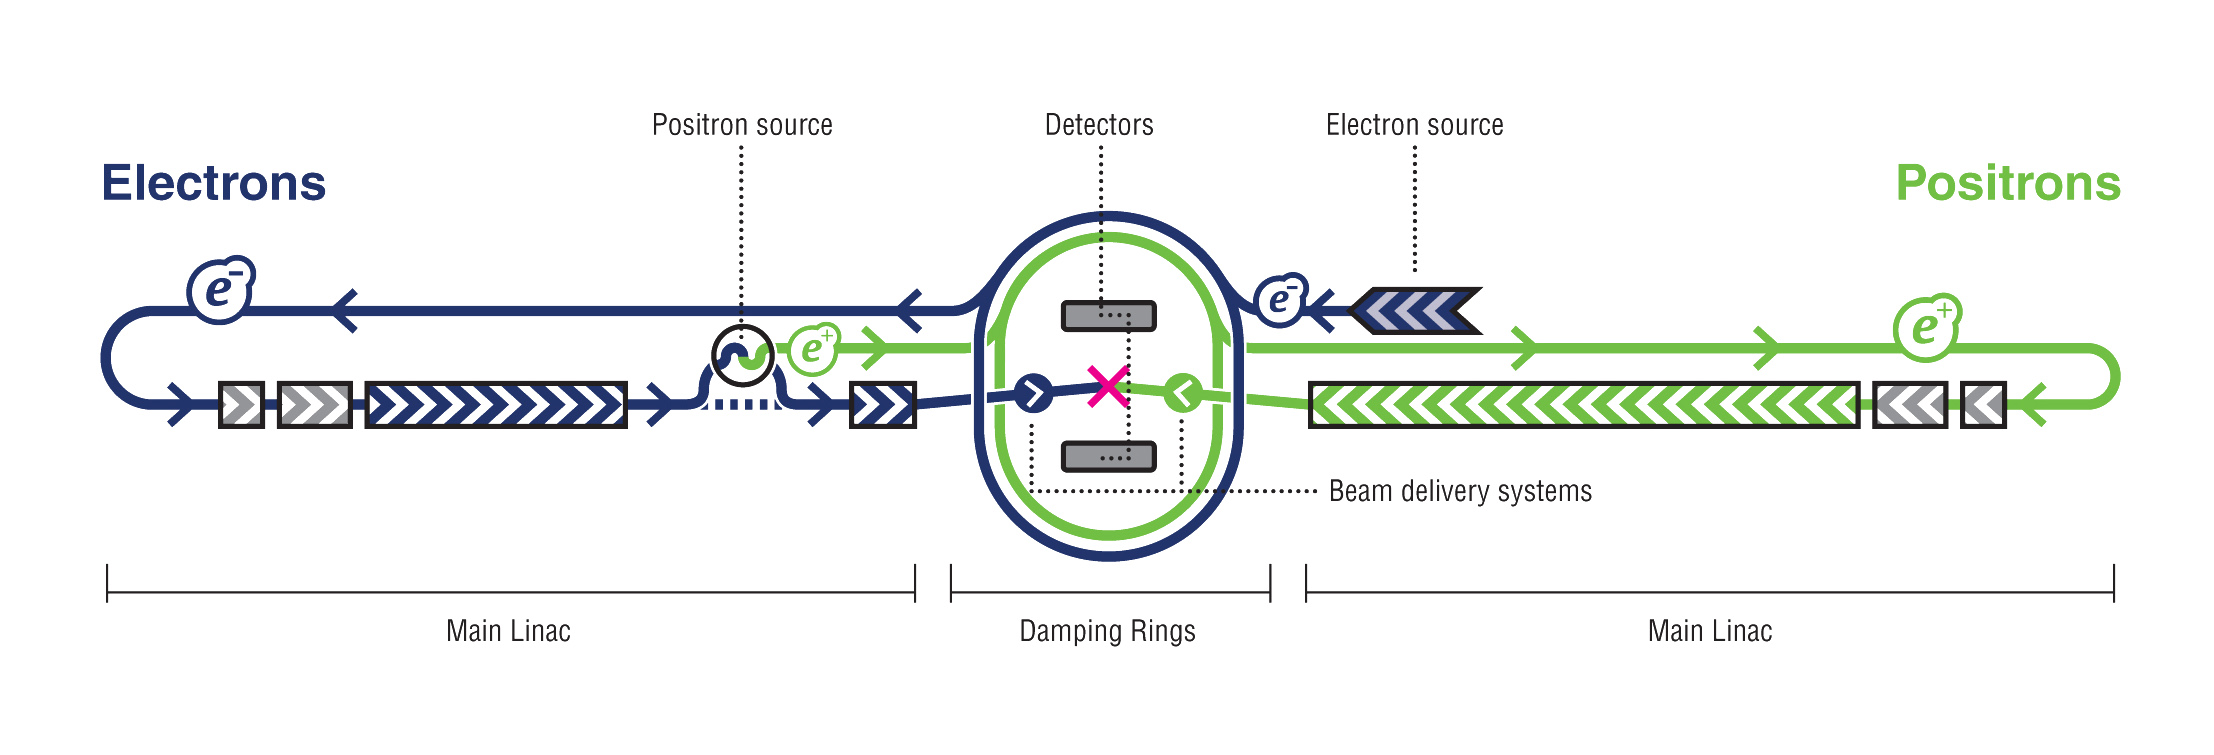
\includegraphics[width=0.95\linewidth]{../graphics/ILC_scheme.jpg}
%		\caption{\sl Schematic view of the ILC accelerator complex. }
%		\label{fig:ILCScheme}
%	}
%\end{figure}

%The schematic view of the ILC accelerator complex is shown in Fig.~\ref{fig:ILCScheme}.
In this work, the $e^+ e^-\to b\bar{b}$ channel is studied at $\sqrt{s}=250$\,GeV using full simulation of the ILD experiment.
The high-granularity of the ILD subdetectors allows for an individual particle reconstruction using the Particle Flow approach.
The schematic view of the ILD concept and the subdetector layout is presented in Fig.~\ref{fig:ILDScheme}.

\begin{figure}
	{\centering
		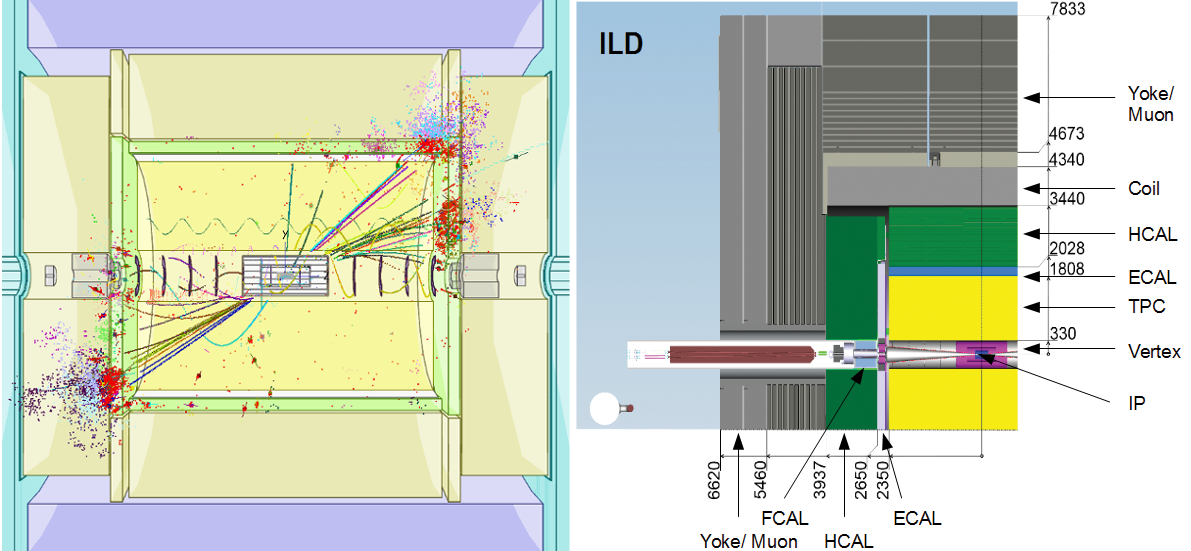
\includegraphics[width=0.8\linewidth]{../poster/figures/ild3.png}
		\caption{\sl Event display of the $e^+ e^-\to b\bar{b}$ process in a full simulation of the ILD detector (left) and schematic view of the ILD concept~\cite{bib:ILC} (right). }
		\label{fig:ILDScheme}
	}
\end{figure}

\section{$b$-quark charge measurement}

The $b$-quark polar angle reconstruction requires an accurate $b$-quark charge measurement. 
The $b$-quark charge is identified using two basic signatures:
\begin{itemize}
	\item \textbf{Vertex charge} is a sum of all reconstructed charges, which are associated to the $b$-hadron vertices. 
	\item \textbf{Kaon charge} is a charge of kaons found in $b$-hadron vertices. 
\end{itemize}

The schematic appearance of $b$-hadron decays in the ILD Vertex Detector is presented in Fig.~\ref{fig:vtx}.

\begin{figure}
	{\centering
		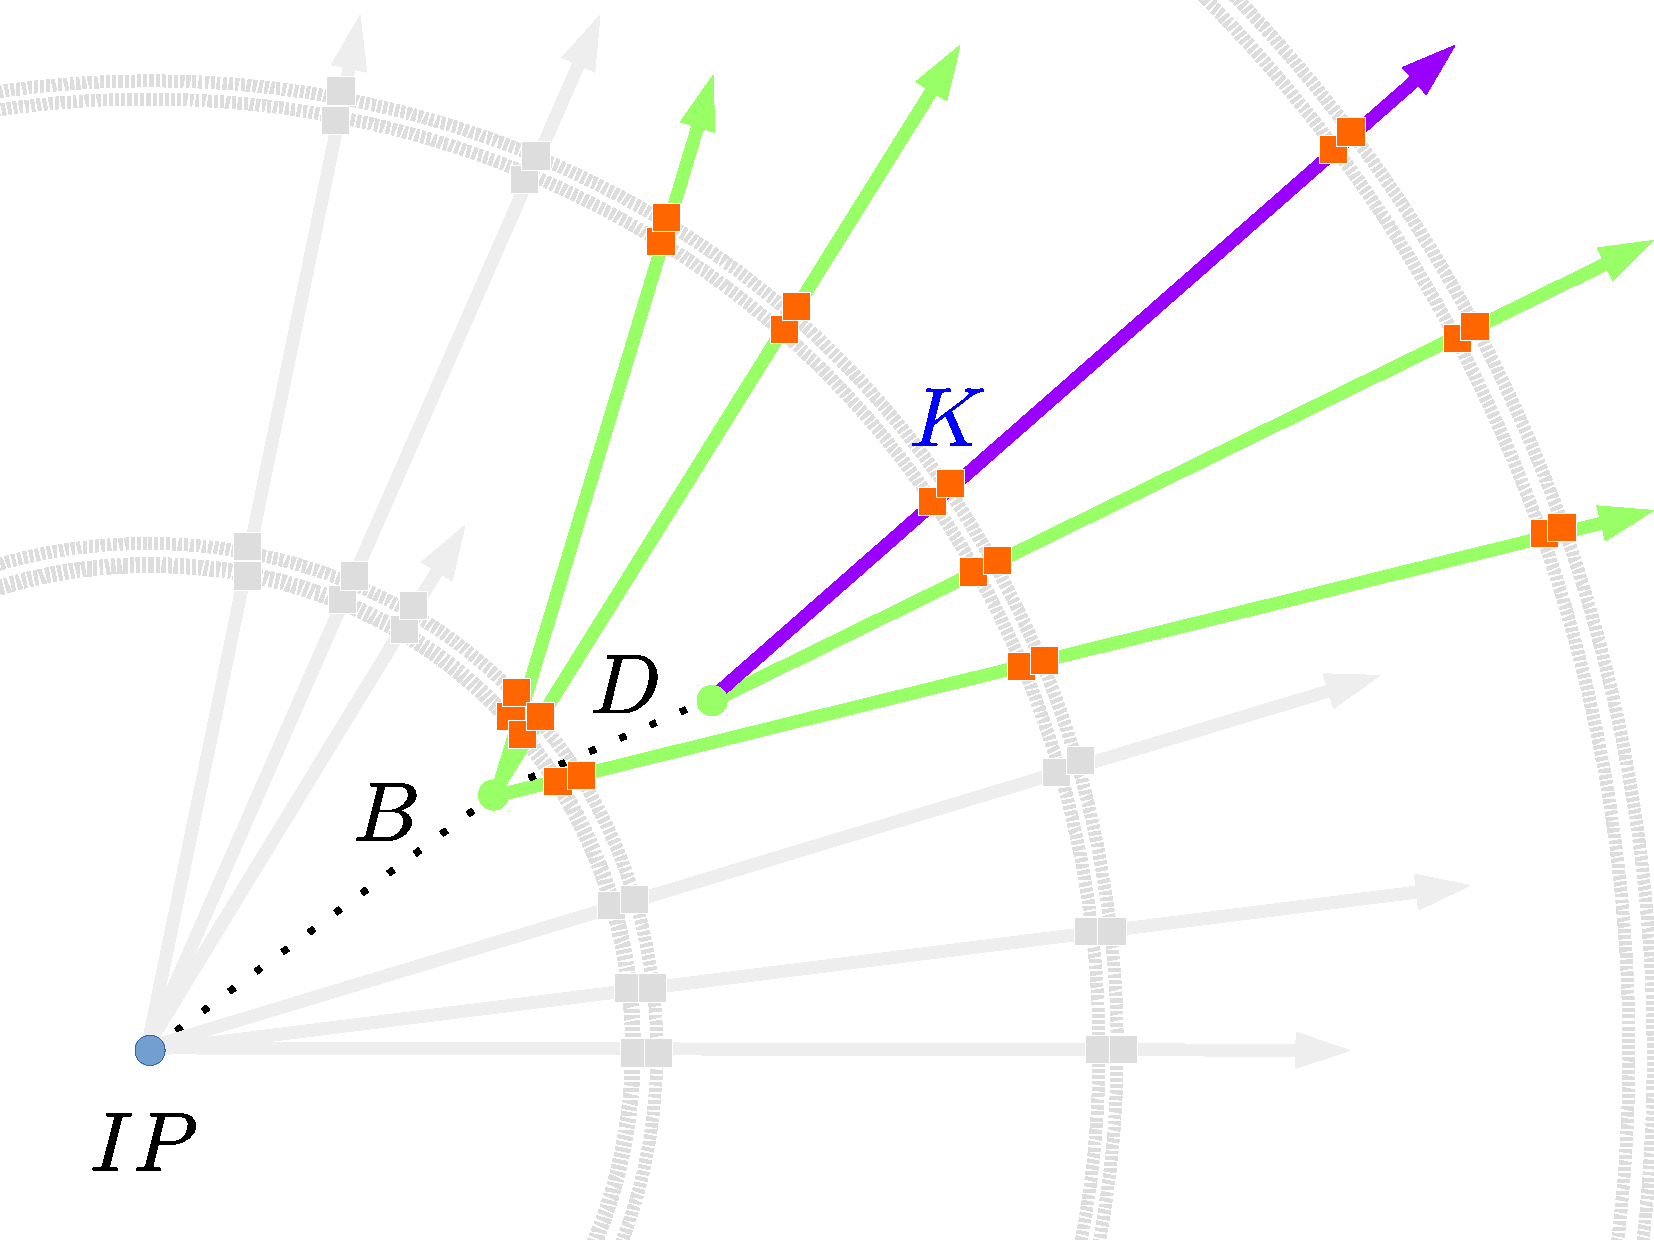
\includegraphics[width=0.45\linewidth]{../poster/figures/vtx.pdf}
		\caption{\sl Illustration of $b$-hadron decays. }
		\label{fig:vtx}
	}
\end{figure}
It was found, that vertexing algorithms can miss one or more b-hadron decay particles from the reconstructed vertices. This effect decreases vertex charge purity.
The developed Vertex Charge Recovery procedure enhances the vertex charge purity by adding the missing b-hadron particles back to the measured vertices using a set of reconstructed observables. 


The kaon identification is possible using the TPC $dE/dx$ information. After equalizing the $dE/dx$ in angular spectrum, the kaons from $b$-hadron vertices can be identified with 97\% purity and 87\% efficiency.

The plots of the vertex charge purity and the $dE/dx$ as function of particle momentum for different hadrons are shown in Fig.~\ref{fig:Charges_3}.

	\begin{figure}
		\centering
		\begin{subfigure}{0.5\textwidth}
			\centering
			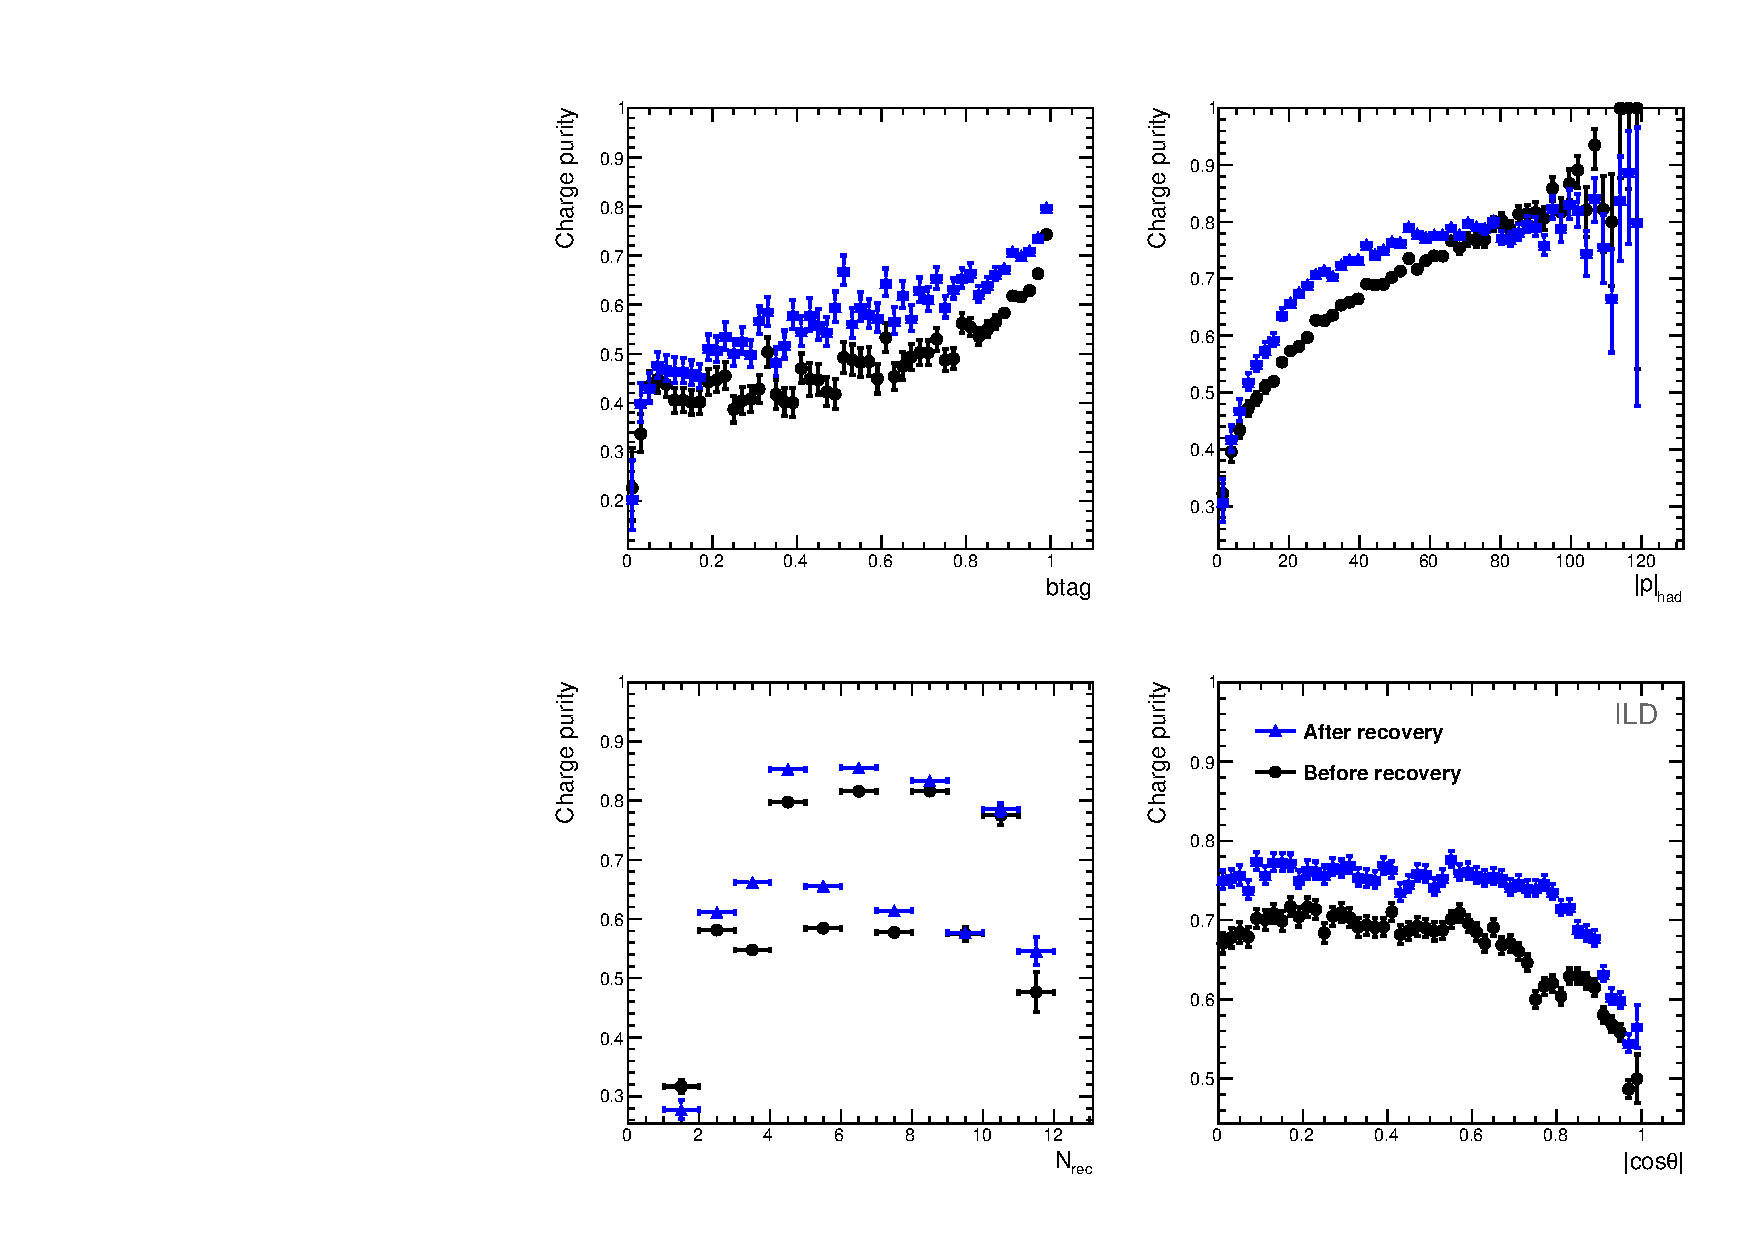
\includegraphics[clip, trim=10cm 0cm 0cm 10cm,width=0.95\linewidth]{../poster/plots/purity-recovery-ild.pdf}
			\caption{\label{fig:thetaepsilonsys} }
		\end{subfigure}% 
		\begin{subfigure}{0.5\textwidth}
			\centering
			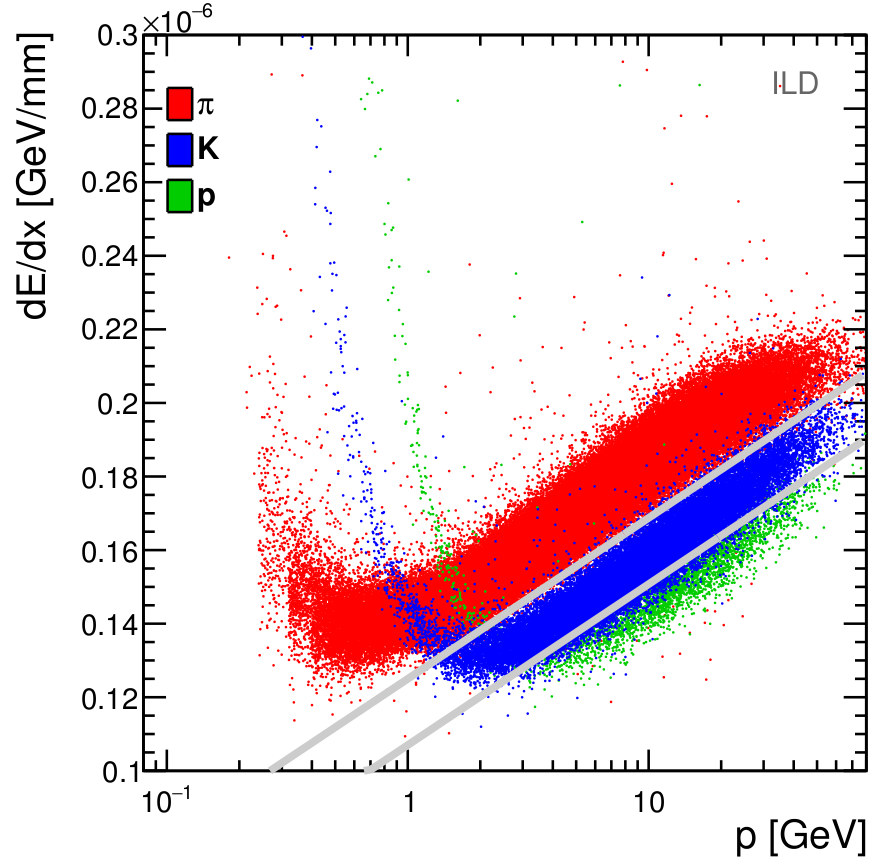
\includegraphics[width=0.87\linewidth]{../poster/plots/dedx2.png}
			\caption{\label{fig:lepsilonsys} }
		\end{subfigure}
		\caption{\label{fig:Charges_3} \sl Vertex charge purity as function of $\cos\theta$ (left) and energy deposition per unit of length $dE/dx$ as function of particle momentum $p$ (right).}
	\end{figure}
	
\section{$b$-quark polar angle spectrum}

The reconstructed b-quark polar angle distributions at $\sqrt{s} = 250$\,GeV using a combination of kaon and vertex charge signatures are demonstrated in Fig.~\ref{fig:BAsymmetryFinal_3}. The integrated luminosity $\mathcal{L}_I = 250$\,fb$^{-1}$ is assumed for each beam polarization.

\begin{figure}
	\centering
	\begin{subfigure}{0.5\textwidth}
		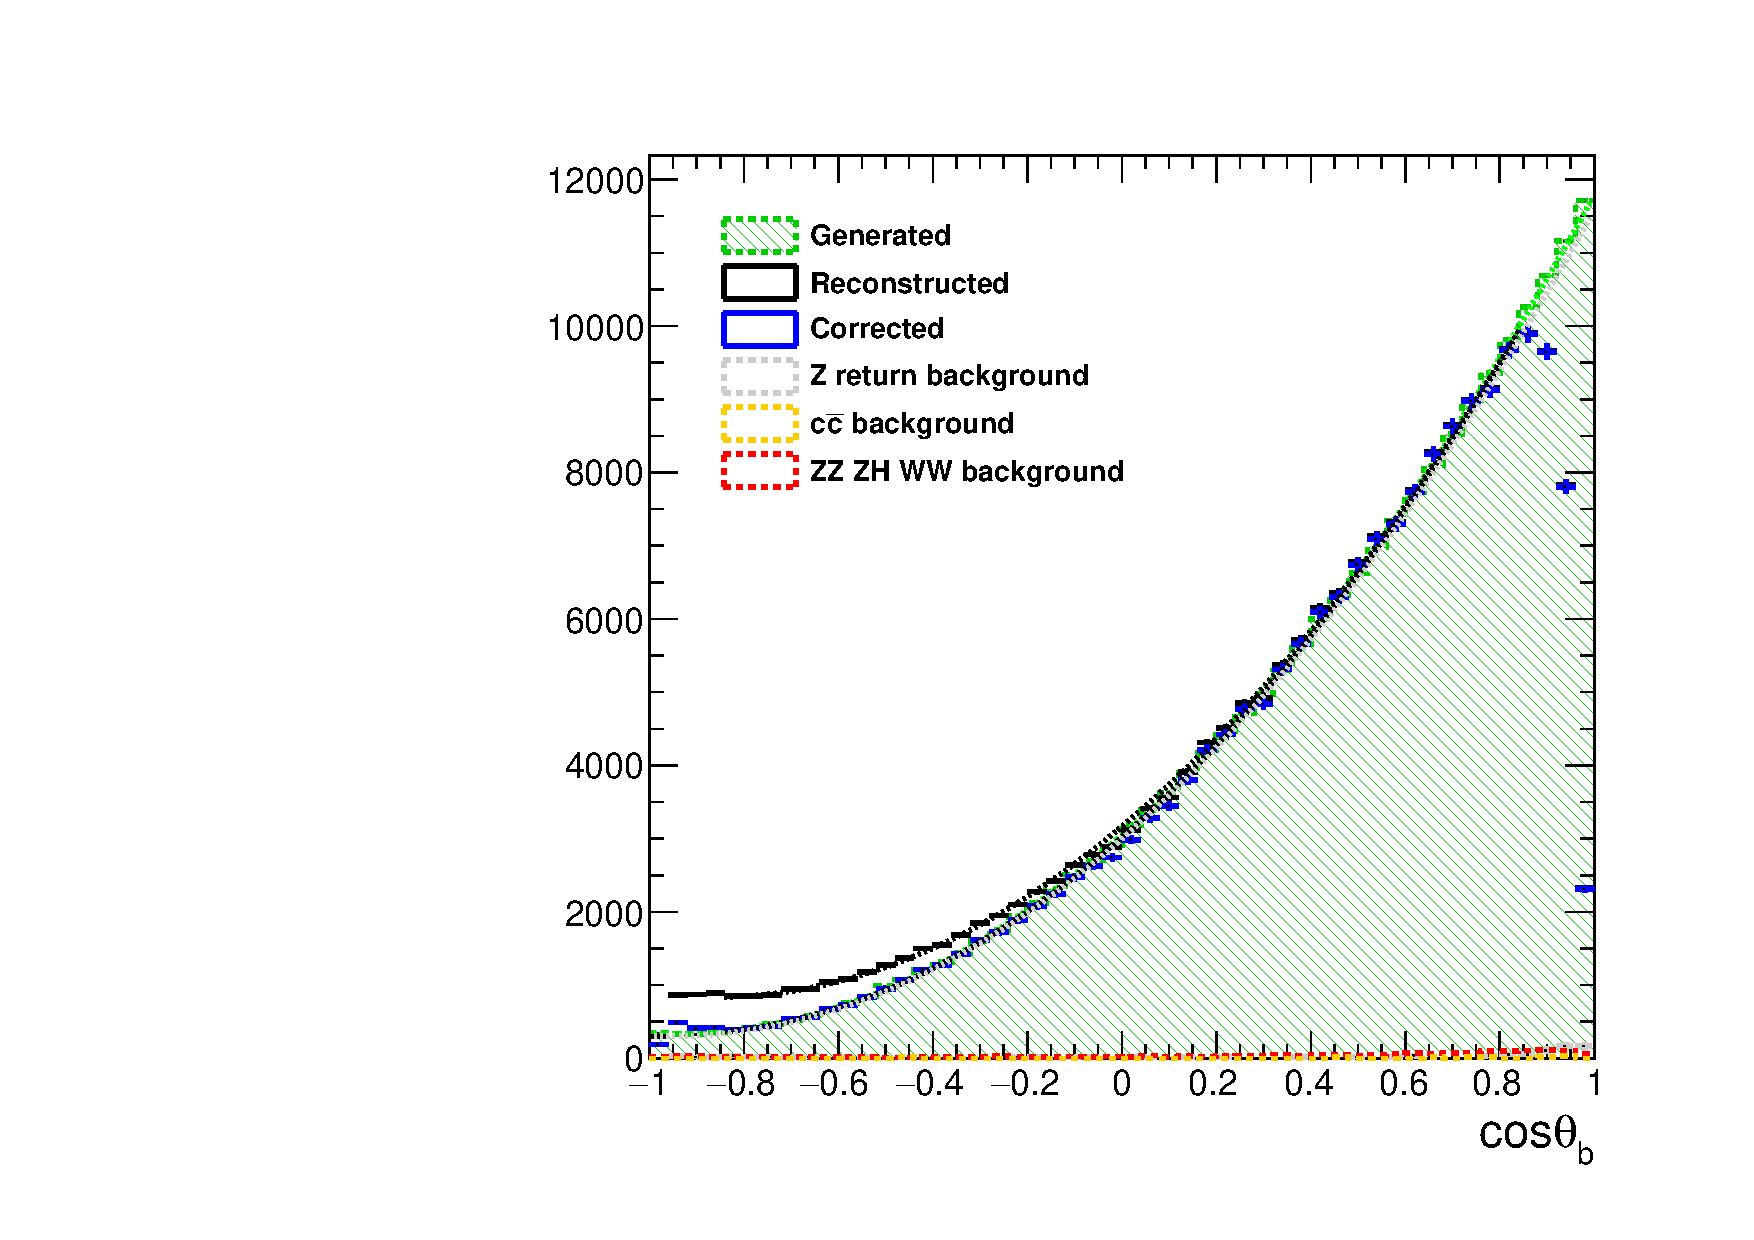
\includegraphics[width=0.95\textwidth]{../ILD/plots/basymmetry-final-left.pdf}
		\llap{\shortstack{%
				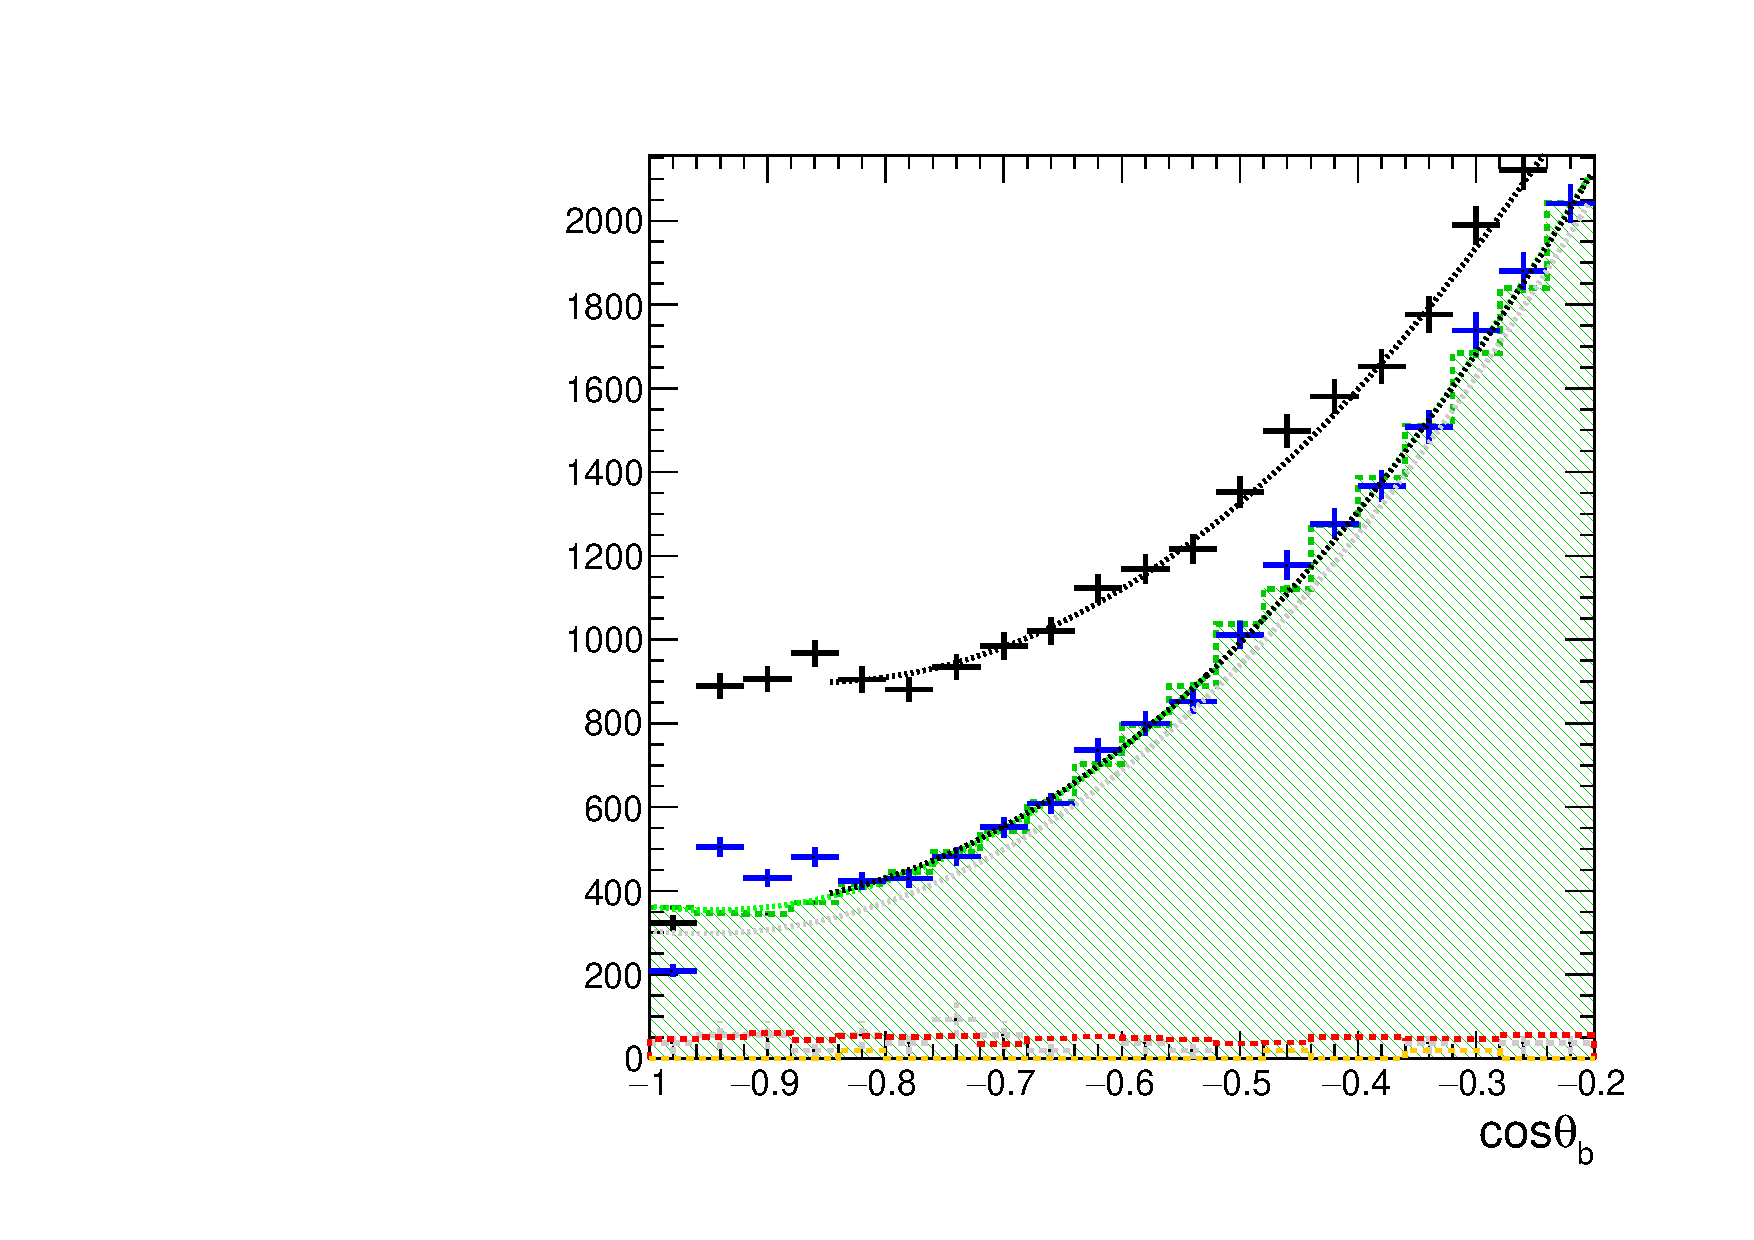
\includegraphics[clip, trim=0cm 0cm 1.8cm 1.7cm, scale=.14]{../ILD/plots/zoom-final.pdf}\\
				\rule{0ex}{0.51in}%
			}
			\rule{1.8in}{0ex}}
		\caption{\label{fig:BAsymmetryFinal_a_3} }
	\end{subfigure}% 
	\begin{subfigure}{0.5\textwidth}
		\centering
		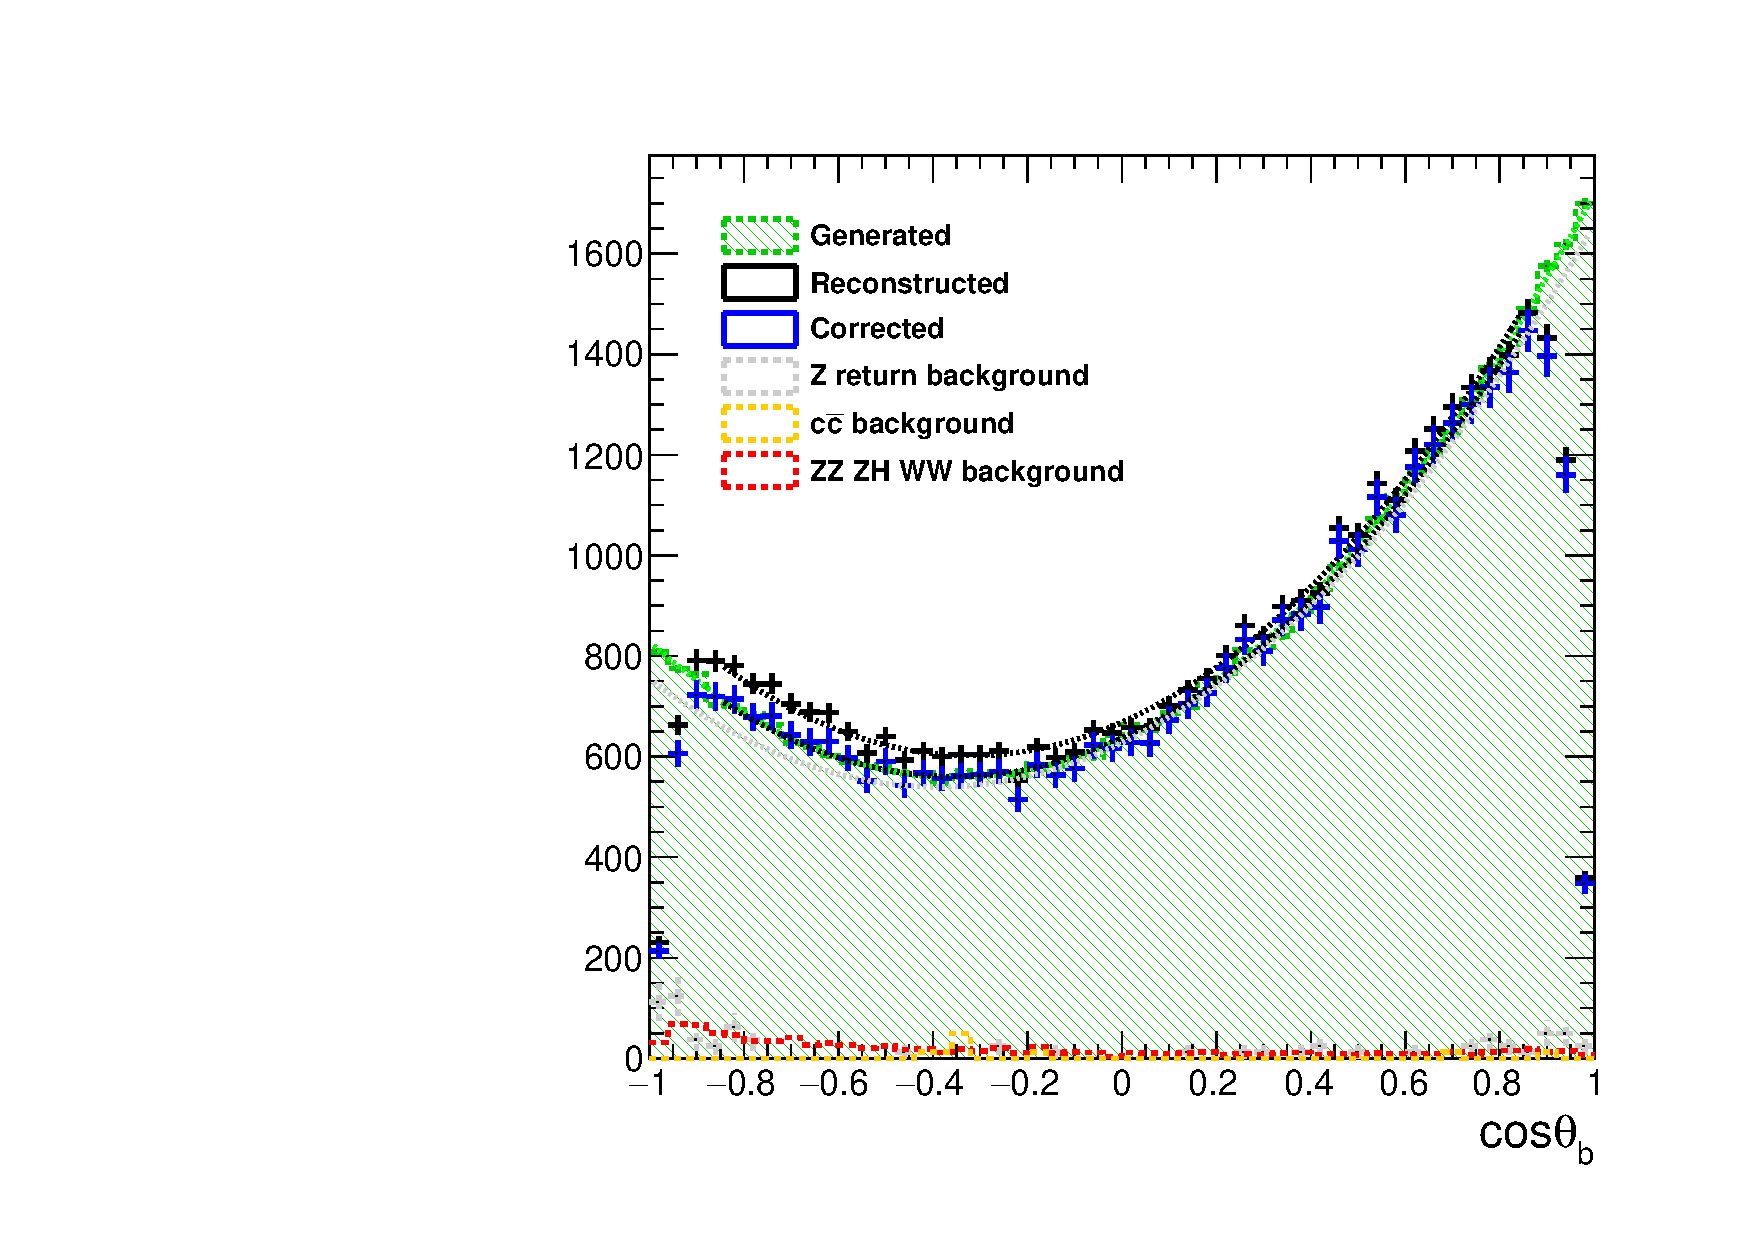
\includegraphics[width=0.95\textwidth]{../ILD/plots/basymmetry-final-right.pdf}
		\caption{\label{fig:BAsymmetryFinal_b_3} }
	\end{subfigure}
	\caption{\sl Generated b-quark polar angle distribution compared to the final reconstructed b-quarks polar angle in left-handed case (a) and right-handed case (b) with overlaid background processes.  }
	\label{fig:BAsymmetryFinal_3}
\end{figure}

The kaon and vertex charge purity is defined using the measured events with misreconstructed charges. Using the measured purities, the reconstructed spectrum is corrected using a data-driven procedure.
The corrected distributions are fitted by a general cross section function, defined as ${	S (1+\cos^2\theta) + A \cos\theta}$. The extracted precision on the $S$ and $A$ parameters is rescaled to the realistic polarization $e^-_L, e^+_R = \pm0.8, \mp0.3$ and the luminosity sharing of the ILC physics program.
As one can see from Fig.~\ref{fig:BAsymmetryFinal_3}, the contribution of the diboson background processes is small. 

\section{Interpretation}

The relative precisions on the $Z^0b\bar{b}$ couplings, $g_L^Z$ and $g_R^Z$, for the LEP~I measurements and for the expected ILC performance are shown in Fig.~\ref{fig:LEPILCResult_3}. 
The ILC precision on the $g_R^Z$ coupling is enough to fully confirm or discard the New Physics influence on the b-quark electroweak couplings. 


\begin{figure}
	\centering
	\begin{subfigure}{0.5\textwidth}
		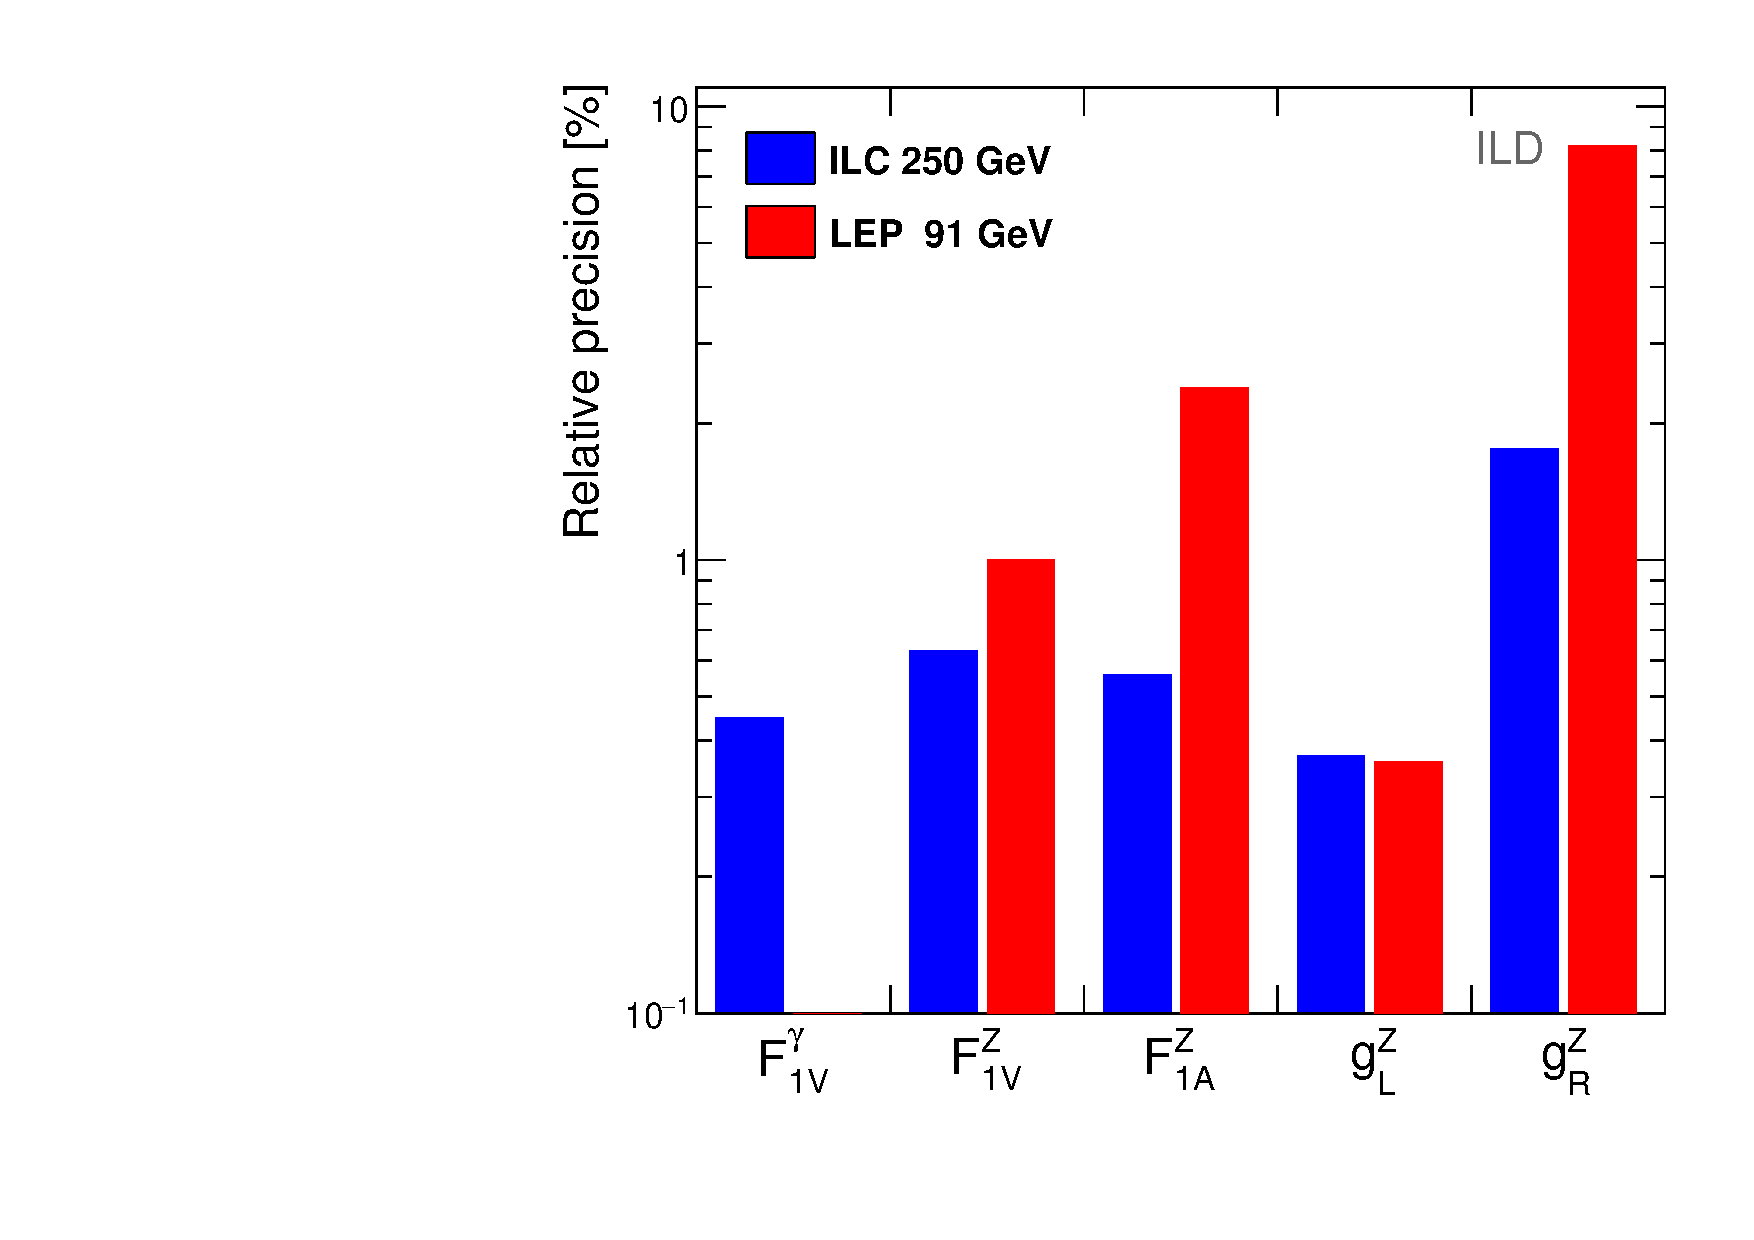
\includegraphics[width=0.95\linewidth]{../poster/plots/final-graph-ild.pdf}
		\caption{\label{fig:LEPILCResult_3_a} }
	\end{subfigure}% 
	\begin{subfigure}{0.5\textwidth}
		\centering
		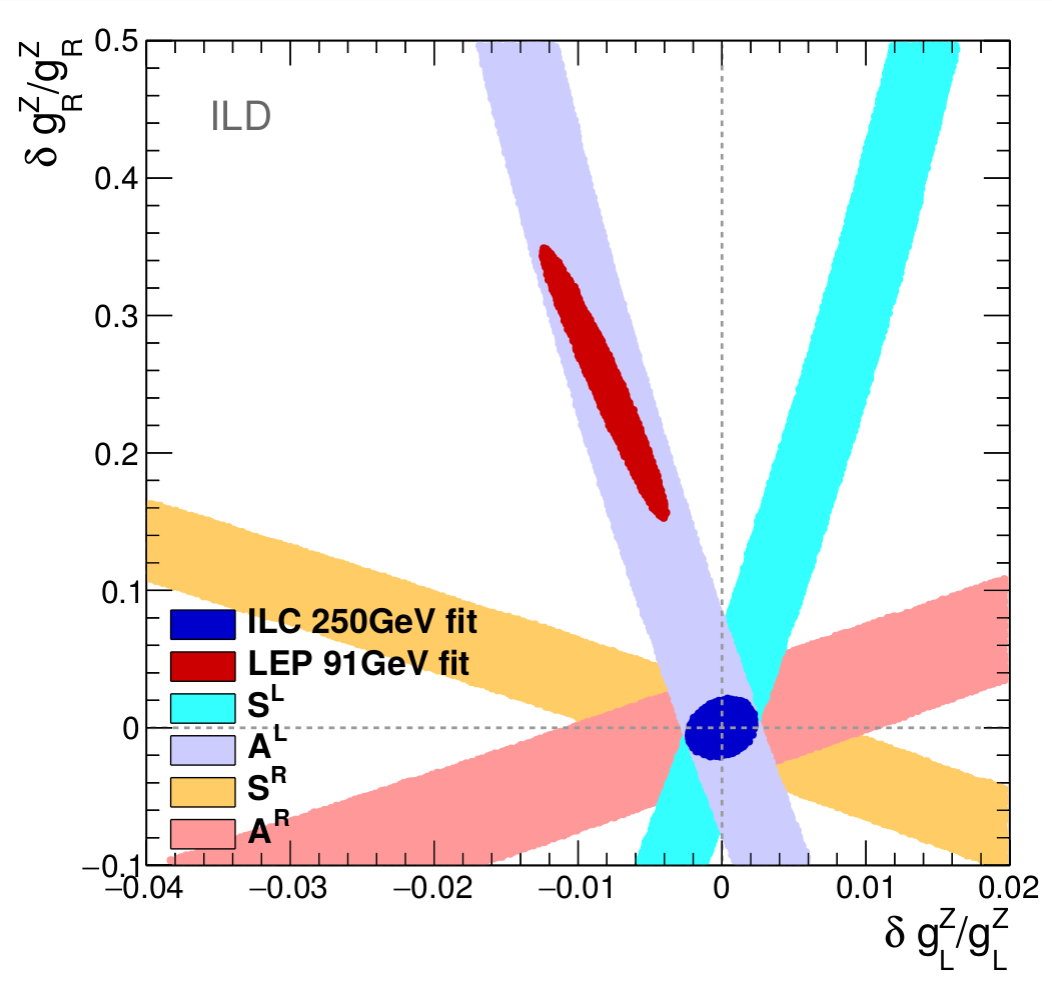
\includegraphics[width=0.95\linewidth]{../poster/plots/ilc-precision-ild.png}
		\caption{\label{fig:LEPILCResult_3_b} }
	\end{subfigure}
	\caption{\sl  Comparison of the LEP measurements to the expected precision at the ILC. The results of the ILC assume an integrated luminosity of $\mathcal{L} = 500$\,fb$^{-1}$ shared between beam polarizations at $\sqrt{s} = 250$\,GeV. }
	\label{fig:LEPILCResult_3}
\end{figure}

%--------------------------------------------------------------------------------
%	CONCLUSIONS
%--------------------------------------------------------------------------------

\section*{Conclusions}

\begin{itemize}
	\item The developed procedure of the $b$-quark charge reconstruction allows for measuring the $b$-quark polar angle. The residual impurity is corrected by a data-driven procedure;
	\item The $b$-quark polar angle fit allows for an independent determination of four electroweak couplings of the $b$-quark. The fit can be extended to include also a term proportional to $\sin^2\theta$, giving access to an independent determination of the tensorial couplings;
	\item  The relative precision on the right-handed coupling $dg^Z_R/g^Z_R\approx 2$\% at the ILC is sufficient to confirm at $>5\,\sigma$ or to discard the LEP~I effect, which is at the 25\% level;
	\item A reach of $\Lambda \approx 10$\,TeV is achievable for indirect New Physics searches.
	%\item The statistical precision after the first $\sqrt{s} = 250\,$GeV ILC program will be almost 5 times better than at LEP;
\end{itemize}


\section*{Forthcoming Research}
The b-quark charge technique was originally developed for the t-quark polar angle measurement in the semileptonic decay channel and it can be applied to the fully hadronic $t\bar{t}$ decays.
The kaon charge method can be extended on the c-quark polar angle analysis, where one can improve the LEP~I results on the c-quark couplings precision. 
Hence, at the ILC one can measure the top, bottom and charm quark electroweak couplings with an excellent sensitivity to New Physics effects.

\section*{Acknowledgements}

These studies are done using the full ILD simulation and we acknowledge the work of the ILD software and simulation groups.



%%%%%%%%%%%%%%%%%%%%%%%%%%%%%%%%%%%%%%%%%%%%%%%%%%%%%%%%%%%%%%%%%%%%%%%%%%%%%%%
\bibliographystyle{unsrt} % Plain referencing style
\bibliography{../mainbib} 
%\begin{thebibliography}{99}
%\bibitem{...}
%....

%\end{thebibliography}

\end{document}
\grid
